\chapter{Introdução}
\label{chap:introducao}

Mais do que nunca observa-se o quão sobrecarregados as pessoas estão com a quantidade de dados que criam a cada dia \cite{Pradeep2017}. Quando compara-se quanto de informação vem sendo gerada nos ultimos anos, percebe-se que está aumentando significamente. Além dessa evolução quantitativa, hoje, encontra-se os mais diversos tipos de informação, por exemplo: documentos, tuítes, fotos, vídeos, \textit{GIFs}, \textit{check-ins} entre vários outros.

Esse fenômeno vem sido chamado de \textit{Big Data} e representa uma crescente área de estudo atualmente. Como consequência, pesquisadores estão analisando e aprendendo com essas informações geradas, entretanto o crescimento contínuo da quantidade de dados dificulta as análises. Portanto pessoas estão investindo em novas técnicas e ferramentas para romper desafios como mineração de dados, {\em data cleaning}, visualização de dados, classificação de dados, exploração de dados e muito mais \cite{Zhang2015}.

Um tipo comum de dado é chamado de dado espacial, o qual  possui atributos geográficos como latitude e longitude como, por exemplo, tuítes, avaliação de restaurantes, {\em check-ins} em estabelecimentos. Dados espaciais podem ser muito significativos, por exemplo, um {\em check-in} no aeroporto por sua irmã na manhã do seu aniversário, provavelmente significa que você terá uma surpresa.

Cada registro de dados espaciais representa uma atividade numa precisa localização geográfica, em outras palavras, a análise desse tipo de dado permite realizar descobertas baseadas em fatos. Analistas estão frequetemente interessados em observar padrões espaciais e tendências para melhorar seus processos de tomada de decisão. Análise de dados espaciais tem várias aplicações como gerenciamento de cidade inteligentes, gerenciamento de disastres e transporte autônomo \cite{RoddickEHPS04,Telang:2012}.

\section{Problema}

A análise de dados espaciais geralmente é realizada num contexto exploratório: o analista não tem uma consulta precisa em mente e ele explora os dados em passos iterativos a fim de encontrar resultados potencialmente interessantes. Tradicionalmente, um cenário de análise exploratória é descrito na seguinte maneira: o analista visualiza um subconjunto de dados usando uma consulta em ambiente de visualização (por exemplo: Tableau\footnote{\it http://www.tableau.com},
Exhibit\footnote{\it http://www.simile-widgets.org/exhibit/},
Spotfire\footnote{\it http://spotfire.tibco.com}); o resultado será ilustrado em um mapa geográfico; então o analista investiga diferentes partes do conjuto de dados movendo ou focando uma região do mapa afim de encontrar padrões ou tendências de interesse. O analista pode iterar por esse processo várias vezes realizando consultas diferentes e focando em diferentes aspectos.

Contudo, a vasto tamanho do conjunto de dados espacias faz com que o analista se sinta perdido durante a exploração. É possível ter milhares de pontos geográficos em cada bairro de uma cidade, por exemplo. Analistas precisam ter acesso apenas a algumas opções (chamadas de {\em ``highlights''}) que ajam como uma direção e assim permitir que ele foque no que lhe interessa na análise. No cenário perfeito, essas opções não são aleatoriamente escolhidas e representam o que o analista se mostrou interessado em iterações passadas.

Este trabalho formula um modelo para permitir o ``realçamento de dados usando feedback coletado ao longo do tempo''. Em outras palavras, busca-se realçar alguns pontos geográficos baseado nos interesses do analista afim de guiá-lo na direção ao que ele deve se concentrar nas iterações seguintes do processo de análise.

\subsection{Caso de Estudo}

\todo{Checkpoint: alterar para terceira pessoa}

Nessa seção, apresenta-se um caso de estudo afim de demostrar a funcionalidade da abordagem proposta na prática.

\begin{figure}[t]
	\centering
	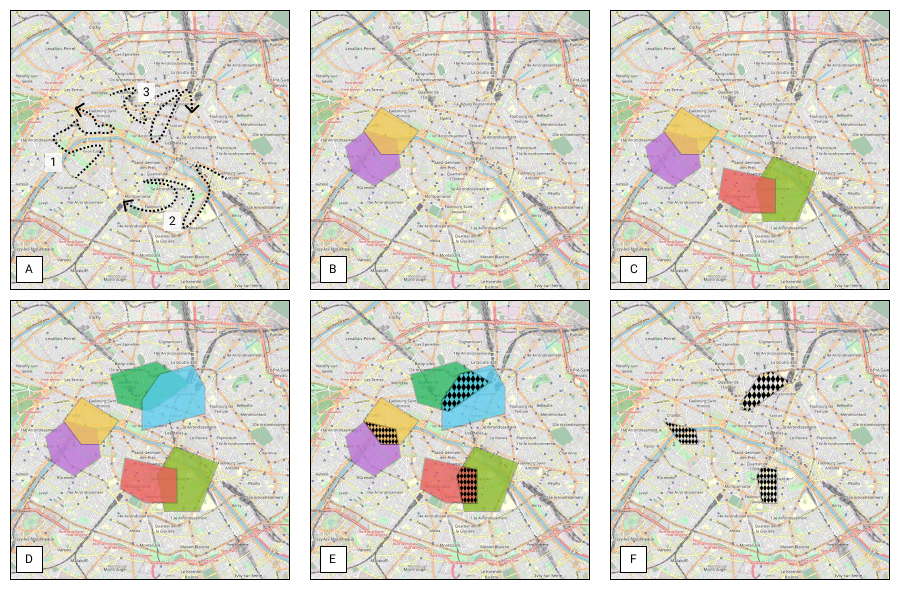
\includegraphics[width=\textwidth]{imagens/caso-de-estudo}
	\caption{Processo de explorar estadias em Paris}
	\label{fig:regions}
\end{figure}

{\bf Exemplo.} {\em Benício está planejando passar alguns dias em Paris, França. Sua apreciação pela cultura francesa faz como que ele tenha interesse em novas experiências na cidade. Ele decidiu por alugar uma estadia pelo Airbnb \footnote{\it http://www.airbnb.com}. Ele gosta de descobrir a cidade, portanto ele é aberto a qualquer tipo de estadia em qualquer região com um leve interesse em ficar perto do centro da cidade. O sistema retorna $4000$ opções diferentes. Como ele não tem outras preferências, uma investigação exaustiva para avaliar cada região da cidade independentemente é necessário, o que é quase impossível. Enquanto estava avaliando algumas opções, ele demostrou interesse na região de  ``Champ de Mars'' (próximo à Torre Eiffel), mas ele esqueceu ou não achou necessário clicar num ponto nessa região. Coletando o feedback do seus movimentos com o mouse no mapa de estadias em Paris, nosso sistema consegue de maneira transparente detectar o interesse dele na região supracitada e apresentar uma quantidade pequena de opções recomendadas para Benício.}

Seguimos o exemplo acima para descrever como feedback implícito é coletado na prática. Imagem \ref{fig:regions} mostra os passos de Benício para explorar estadias em Paris. Imagem \ref{fig:regions}.A mostra os movimentos do mouse dele em diferentes intervalos de tempo. Nesse exemplo, coletamos o feedback de Benício em 3 diferentes intervalos de tempo (evoluindo das Imagens \ref{fig:regions}.B até \ref{fig:regions}.D). Isso mostra que Benício começou sua busca perto da Torre Eiffel e {\em Arc de Triomphe} (Imagem \ref{fig:regions}.B) e gradualmente mostrou também interesse no sul (Imagem \ref{fig:regions}.C) e norte (Imagem \ref{fig:regions}.D). Todas as interseções entre essas regiões são descobertas (regiões tachadas na Imagem \ref{fig:regions}.E), o que representa um conjunto de regiões onde o interesse de Benício está direcionado e onde, provalvemente, ele vai decidir ficar durante sua visita à Paris.

E se Benício quiser voltar para Paris próximo ano? Ele teria que repetir a mesma análise exploratória, a não ser que ele lembre a localização exata das estadias interessantes à ele no ano passado. Usando nosso sistema, ele não precisaria lembrar, porque suas preferências foram coletadas e poderiam ser usadas para realçar um subconjunto similar ao do ano anterior.

No contexto da análise explorátoria, o analista talvez mude suas preferências entre as sessões (por exemplo, no inverno, Benício talvez queira ficar próximo ao Torre Eiffel, mas no verão, ele talvez queira ficar mais distante dos pontos turísticos). Afim de atacar esse desafio, nosso modelo permite uma análise temporal para identificar padrões em como as preferências dos analistas mudam entre as sessões o que permite nosso método de realçamento ser mais preciso e consistente com o interesse do analista mesmo em momentos diferentes do ano.

\section{Objetivos}

Nessa seção, definimos os objetivos gerais e específicos do nosso trabalho.

\subsection{Objetivo Gerais}

\begin{itemize}
	\item Propor um modelo de análise espaço-temporal para orientação na exploração de dados espaciais;
	\item Elaborar como análise temporal pode ser efetivamente aplicada na exploração de dados espaciais.
\end{itemize}

\subsection{Objetivos Específicos}

\begin{itemize}
	\item Descrever o conceito de Região Densas Interessantes usado para captura de feedback;
	\item Apresentar como o modelo de dados por ser aplicado no contexto da análise exploratória;
	\item Descrever o modelo de dados usado para análise temporal;
	\item Investigar como o modelo proposto pode ser explorado no contexto espacial e no contexto de domínio.
\end{itemize}

\section{Organização}

Os próximos capítulos estão organizados na seguinte maneira: no Capítulo \ref{chap:contextualizacao} discutimos o estado da arte por trás desse trabalho; Capítulo \ref{chap:modelo} define o modelo de dados, apresenta como é feito a coleta de feedback durante a análise exploratória, demostra como a análise temporal pode ser aplicada. Capítulo \ref{chap:conclusao} conclui e propôe futuros trabalhos.
